% =====================================================================
% Apêndice A -- Matriz bruta de infraestrutura dos pontos P01--P10
%   Reprodução em LaTeX da planilha de levantamento de campo.
%   Versão v3: tabela única em paisagem com coordenadas integradas,
%   mapa do Campus 2 com pontos marcados, legendas breves.
% =====================================================================

\chapter{Matriz bruta de infraestrutura dos pontos P01--P10}
\label{ap:matriz-pontos}

A Tabela~\ref{tab:matriz-pontos} reproduz, em formato tabular, a matriz bruta de levantamento de infraestrutura dos dez pontos candidatos a instalação de câmeras de \textit{camera trapping} no Campus~2 da USP São Carlos. Cada linha corresponde a um ponto identificado durante o reconhecimento de campo conduzido em conjunto com voluntários da AEX Gatos do C2. As colunas registram atributos físicos do local (cobertura, iluminação, edifício), atributos operacionais (movimento de pessoas, vandalismo), atributos de infraestrutura técnica (tomada elétrica, cobertura Wi-Fi USP, cobertura 4G, insolação direta para painel solar, presença prévia de câmeras de segurança institucionais e presença de outros animais) e as coordenadas geográficas aproximadas obtidas por GPS de telefone celular. A Figura~\ref{fig:mapa-pontos} apresenta a distribuição espacial dos dez pontos sobre o mapa do Campus~2. Essa matriz alimenta a discussão de tipologias do Capítulo~\ref{cap:hardware} e a decisão arquitetural consolidada na Seção~\ref{sec:decisao-arquitetural}.

\begin{landscape}
\begin{footnotesize}
\setlength{\tabcolsep}{3pt}
\renewcommand{\arraystretch}{1.15}
\begin{longtable}{@{}p{0.5cm}p{2.8cm}p{1.9cm}p{1.3cm}p{1.1cm}p{1.1cm}p{0.9cm}p{0.6cm}p{0.9cm}p{0.8cm}p{0.5cm}p{0.7cm}p{0.7cm}p{0.7cm}p{1.5cm}p{1.5cm}@{}}
\caption[Formulário de campo dos pontos P01--P10 preenchido com voluntários da AEX Gatos do C2]{Formulário de campo dos pontos P01--P10 preenchido com voluntários da AEX Gatos do C2.}
\label{tab:matriz-pontos}\\
\toprule
\textbf{ID} & \textbf{Local} & \textbf{Edifício} & \textbf{Cobert.} & \textbf{Luz not.} & \textbf{Mov.} & \textbf{Vand.} & \textbf{Tom.} & \textbf{Dist.\ tom.} & \textbf{Wi-Fi USP} & \textbf{4G} & \textbf{Sol $>$4h} & \textbf{Câm.\ seg.} & \textbf{Outros anim.} & \textbf{Latitude} & \textbf{Longitude} \\
\midrule
\endfirsthead
\multicolumn{16}{c}{{\bfseries Tabela~\thetable\ -- Continuação da página anterior}} \\
\toprule
\textbf{ID} & \textbf{Local} & \textbf{Edifício} & \textbf{Cobert.} & \textbf{Luz not.} & \textbf{Mov.} & \textbf{Vand.} & \textbf{Tom.} & \textbf{Dist.\ tom.} & \textbf{Wi-Fi USP} & \textbf{4G} & \textbf{Sol $>$4h} & \textbf{Câm.\ seg.} & \textbf{Outros anim.} & \textbf{Latitude} & \textbf{Longitude} \\
\midrule
\endhead
\midrule \multicolumn{16}{r}{{Continua na próxima página}} \\
\endfoot
\bottomrule
\endlastfoot
P01 & Atrás cantina Eng.\ Comp.     & Eng.\ Comp.    & Semi-coberto & Fraca   & Médio       & Baixo & Sim & 5\,m  & Sim & Sim & Sim & Sim & Sim & $-22{,}004900$ & $-47{,}933700$ \\
P02 & Atrás prédio Eng.\ Comp.      & Eng.\ Comp.    & Aberto       & Fraca   & Quase nulo  & Baixo & Não & ---   & Sim & Sim & Sim & Não & Sim & $-22{,}004900$ & $-47{,}933450$ \\
P03 & Atrás Anfiteatro              & Bloco didático & Aberto       & Fraca   & Médio       & Baixo & Não & ---   & Sim & Sim & Sim & Não & Sim & $-22{,}002217$ & $-47{,}930883$ \\
P04 & Lado Anfiteatro               & Bloco didático & Semi-coberto & Boa     & Alto        & Médio & Não & ---   & Sim & Sim & Sim & Não & Sim & $-22{,}002300$ & $-47{,}931183$ \\
P05 & Corredor Anfiteatro / WCs     & Bloco didático & Coberto      & Ausente & Alto        & Médio & Sim & 10\,m & Sim & Sim & Não & Não & Sim & $-22{,}001217$ & $-47{,}931500$ \\
P06 & Corredor Biblioteca           & Biblioteca     & Coberto      & Boa     & Alto        & Médio & Sim & 5\,m  & Sim & Sim & Sim & Não & Sim & $-22{,}001733$ & $-47{,}931583$ \\
P07 & Entre prédios Bloco Laranja   & Bloco didático & Semi-coberto & Boa     & Baixo       & Baixo & Não & ---   & Sim & Sim & Sim & Não & Sim & $-22{,}002100$ & $-47{,}931350$ \\
P08 & Bloco Amarelo / Entre prédios & Bloco didático & Semi-coberto & Fraca   & Quase nulo  & Baixo & Não & ---   & Sim & Sim & Sim & Não & Sim & $-22{,}001967$ & $-47{,}931467$ \\
P09 & Atrás prédio Aero 1           & Aeronáutica    & Aberto       & Ausente & Quase nulo  & Baixo & Não & ---   & Sim & Sim & Sim & Não & Sim & $-22{,}002367$ & $-47{,}932450$ \\
P10 & Atrás prédio Aero 2           & Aeronáutica    & Aberto       & Fraca   & Quase nulo  & Baixo & Não & ---   & Sim & Sim & Sim & Não & Sim & $-22{,}002783$ & $-47{,}932183$ \\
\end{longtable}
\par\vspace{-0.5em}
\noindent\footnotesize\textbf{Fonte:} Levantamento de campo realizado pelo autor em conjunto com voluntários da AEX Gatos do C2.
\end{footnotesize}
\end{landscape}

\begin{figure}[!htb]
\centering
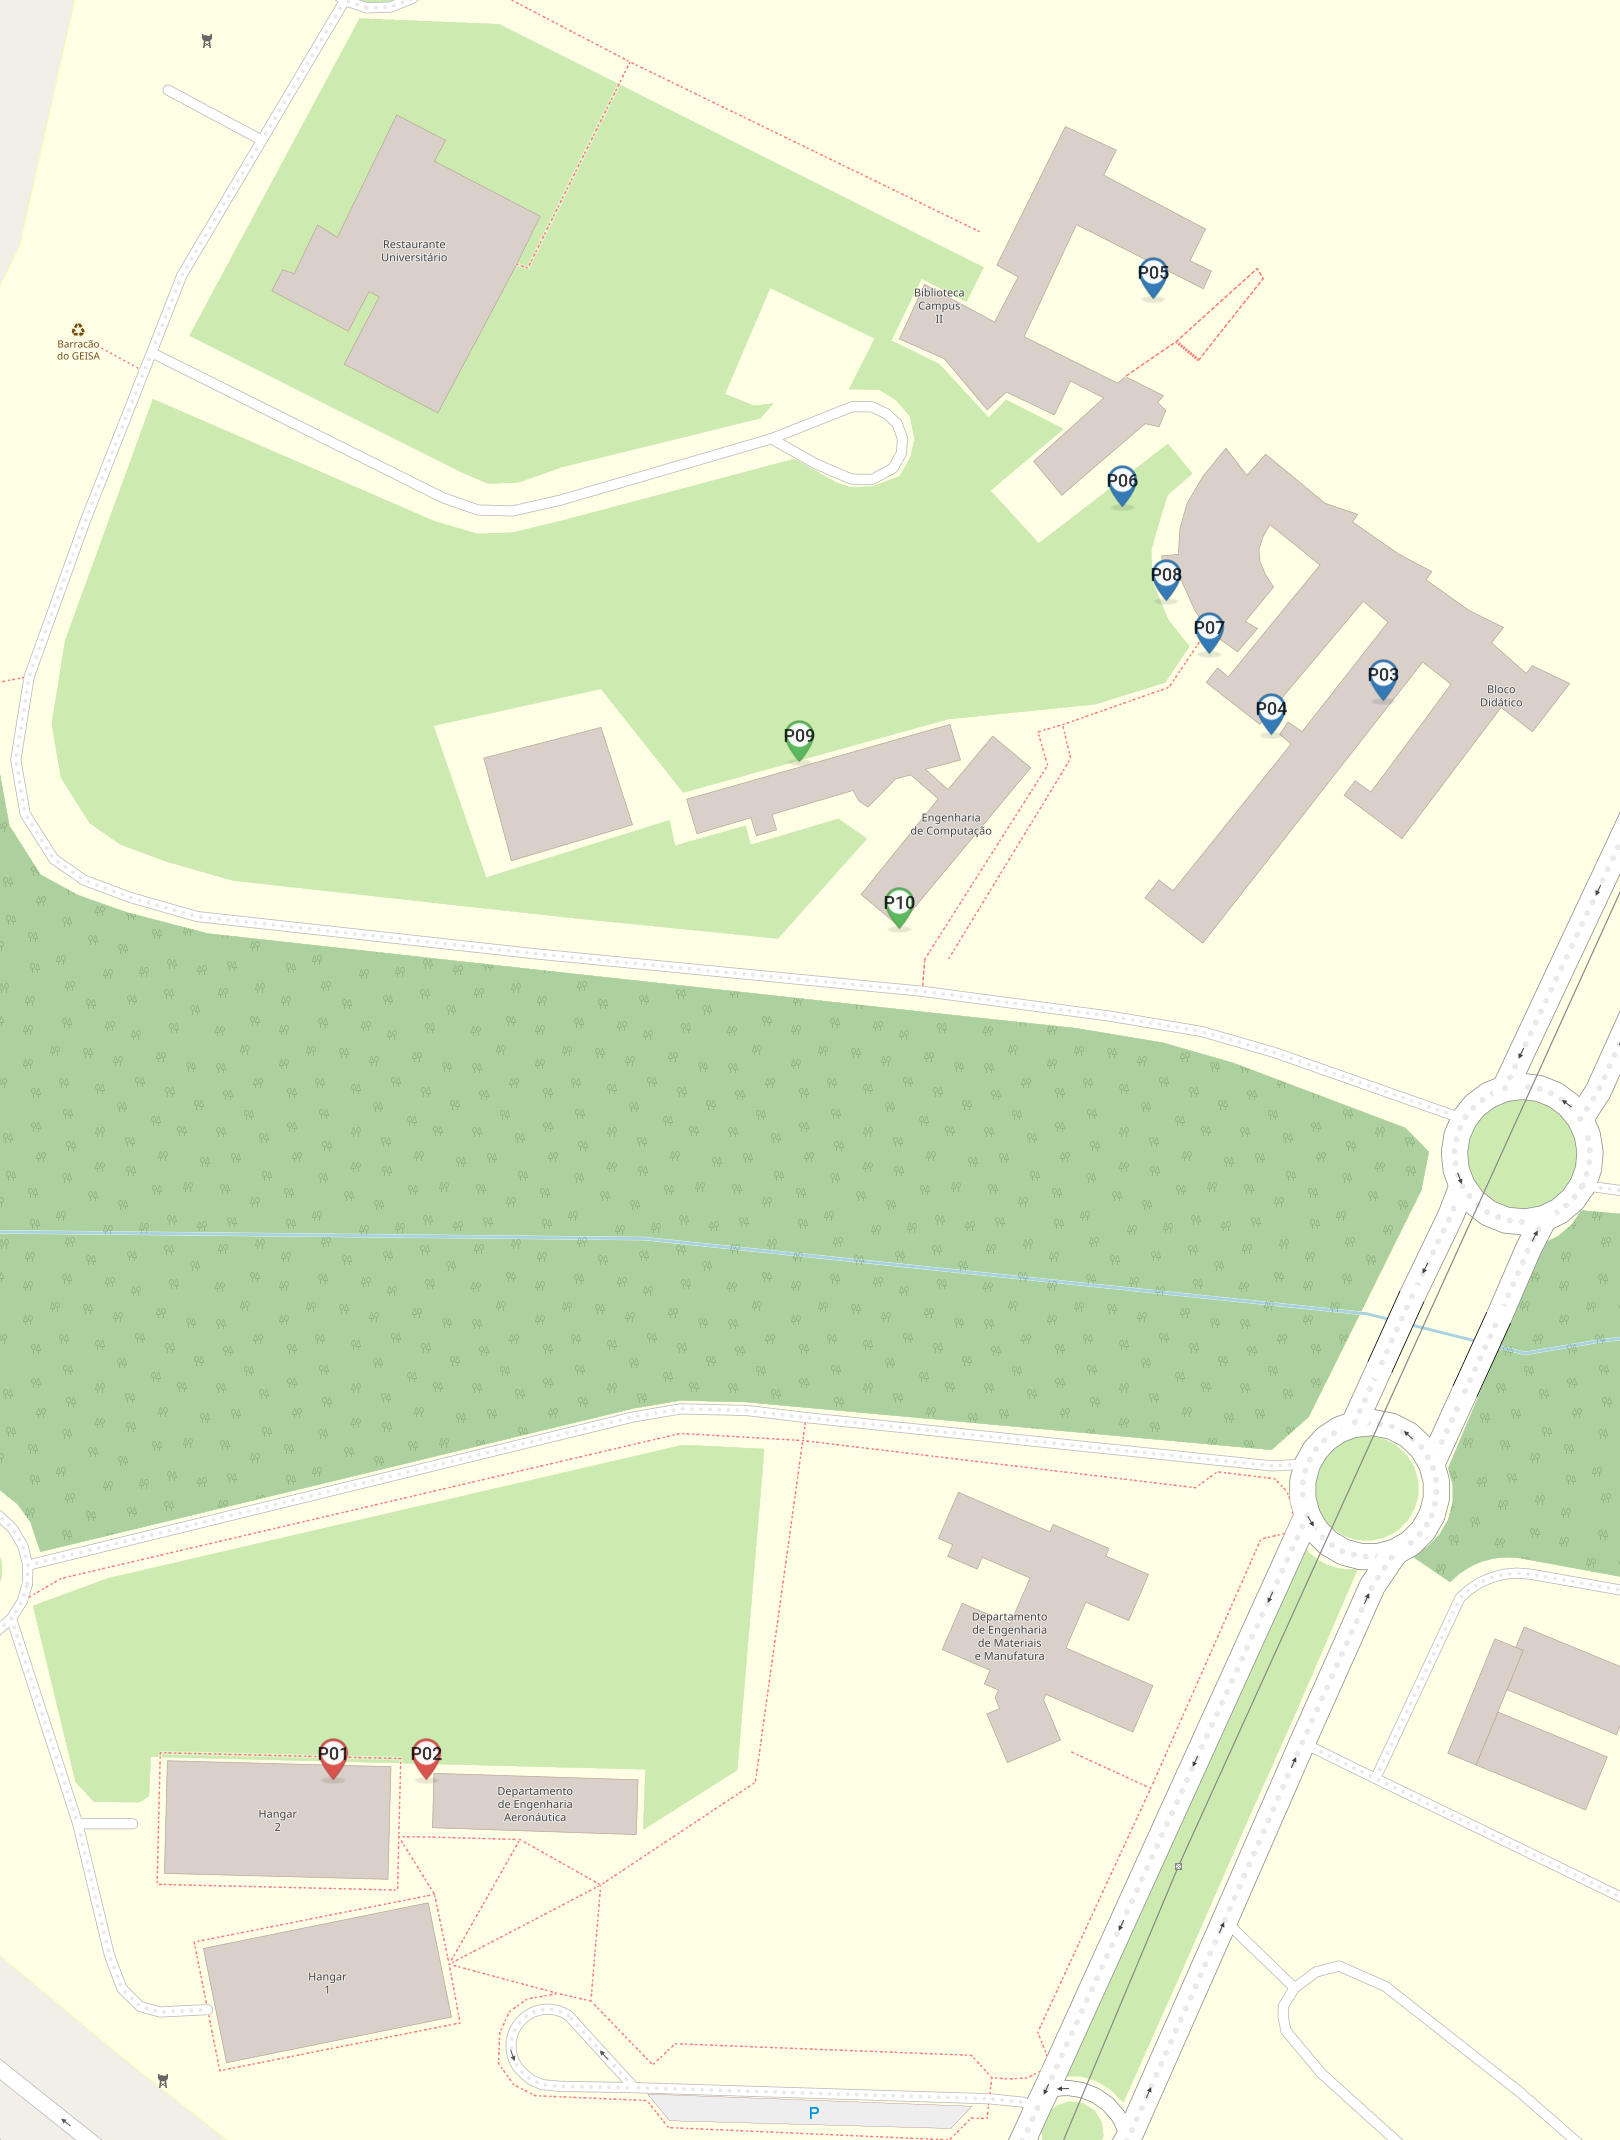
\includegraphics[width=0.85\linewidth]{elementos/figuras/mapac2.png}
\caption[Mapa do Campus~2 com os pontos de alimentação P01--P10]{Mapa do Campus~2 com os pontos de alimentação P01--P10.}
\label{fig:mapa-pontos}
\fonte{Elaborado pelo autor sobre base cartográfica do OpenStreetMap.}
\end{figure}

A leitura cruzada da matriz com a discussão de tipologias revela três agrupamentos operacionais bem definidos. Em primeiro lugar, P01, P05 e P06 são pontos com tomada elétrica próxima, cobertura física e fluxo médio a alto de pessoas, candidatos naturais a tipologia IPCAM com alimentação por rede elétrica e armazenamento em cartão microSD. Em segundo lugar, P02, P03 e P07 a P10 são pontos sem tomada próxima, com cobertura aberta ou semi-coberta e insolação direta suficiente para alimentação por painel solar de pequeno porte, candidatos a câmera autônoma alimentada por bateria. Em terceiro lugar, P04 isola-se como ponto de movimento alto, cobertura semi-coberta e iluminação noturna boa, candidato a tipologia híbrida com possibilidade de instalação de SBC para processamento em borda caso a disponibilidade de tomada seja resolvida pela equipe da Prefeitura do Campus~2. Esses agrupamentos são a base operacional da Seção~\ref{sec:decisao-arquitetural} e devem orientar a escolha de equipamento na fase de implantação.

Cabe registrar que as coordenadas declaradas na Tabela~\ref{tab:matriz-pontos} têm precisão limitada à do GPS do telefone celular utilizado em campo e não devem ser tomadas como referência cartográfica oficial. Uma planta georreferenciada precisa, produzida em conjunto com a Prefeitura do Campus~2 sobre o mapa institucional, permanece prevista como item de implantação.
